\chapter{Constituents of Matter, Nuclear Binding, and Stability}
\label{ch:constituents_nuclear}

\begin{chapterintro}
\textbf{Chapter Objectives:} In this chapter, we explore the subatomic anatomy of the atom and the powerful forces that bind the atomic nucleus. You will trace the experimental discoveries of the electron, proton, and neutron; master nuclide notation for neutral atoms and polyatomic ions; calculate relative atomic masses from mass-spectrometric isotopic abundances; formulate the nuclear mass defect ($\Delta m$); apply Einstein's mass-energy equivalence to compute binding energies ($E_L$); and analyze nuclear stability and exothermic energy release across the Aston binding energy curve.
\end{chapterintro}

\section{The Subatomic Architecture of the Atom}

At the close of the nineteenth century, the atom was transformed from Dalton's idealized, indivisible solid sphere into an intricate composite dynamical system consisting of three fundamental subatomic particles:

\begin{figure}[htbp]
\centering
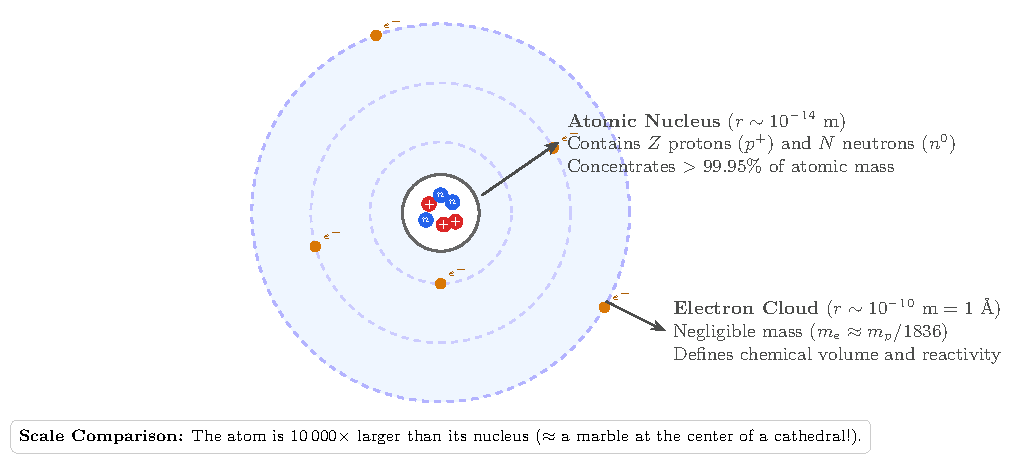
\includegraphics[width=0.74\textwidth]{figures/04_atom_structure.pdf}
\caption{The internal anatomy of the atom. The dense, central nucleus ($r_n \sim 10^{-14}\ \mathrm{m}$) concentrates over $99.95\%$ of total atomic mass, while the surrounding electron cloud ($r_{\text{atom}} \sim 10^{-10}\ \mathrm{m}$) governs atomic volume and chemical bonding.}
\label{fig:atom_structure}
\end{figure}

\subsection{1. Historical Discoveries of Subatomic Particles}
\begin{itemize}[leftmargin=1.5em,itemsep=4pt]
  \item \textbf{The Electron ($e^-$):} Discovered in 1897 by British physicist Joseph John Thomson at the Cavendish Laboratory using cathode ray tubes. By subjecting cathode ray beams to crossed electric and magnetic fields, Thomson measured their charge-to-mass ratio ($e/m_e \approx -1.7588 \times 10^{11}\ \mathrm{C\cdot kg^{-1}}$), proving that cathode rays consist of universal, negatively charged corpuscles possessing less than $1/1800$ the mass of a hydrogen atom.
  \item \textbf{The Proton ($p^+$):} Following his 1911 gold foil scattering experiment which revealed that positive charge is concentrated in a tiny central nucleus, Ernest Rutherford in 1919 bombarded nitrogen gas with energetic alpha particles ($^4_2\mathrm{He}^{2+}$), detecting emitted hydrogen nuclei:
  \[
  \ce{^{14}_7N + ^4_2He -> ^{17}_8O + ^1_1p}.
  \]
  Rutherford named this fundamental positive nuclear particle the \textbf{proton}.
  \item \textbf{The Neutron ($n^0$):} In 1932, James Chadwick irradiated beryllium with alpha particles and observed an intensely penetrating, electrically neutral radiation capable of ejecting high-energy protons from paraffin wax. Chadwick proved these neutral corpuscles were elementary nucleons of mass nearly identical to the proton, completing the nuclear triad.
\end{itemize}

\begin{historicalbox}{J.~J.~Thomson, Rutherford, and Chadwick: Unlocking the Nucleus}
\begin{minipage}{0.30\textwidth}
\centering
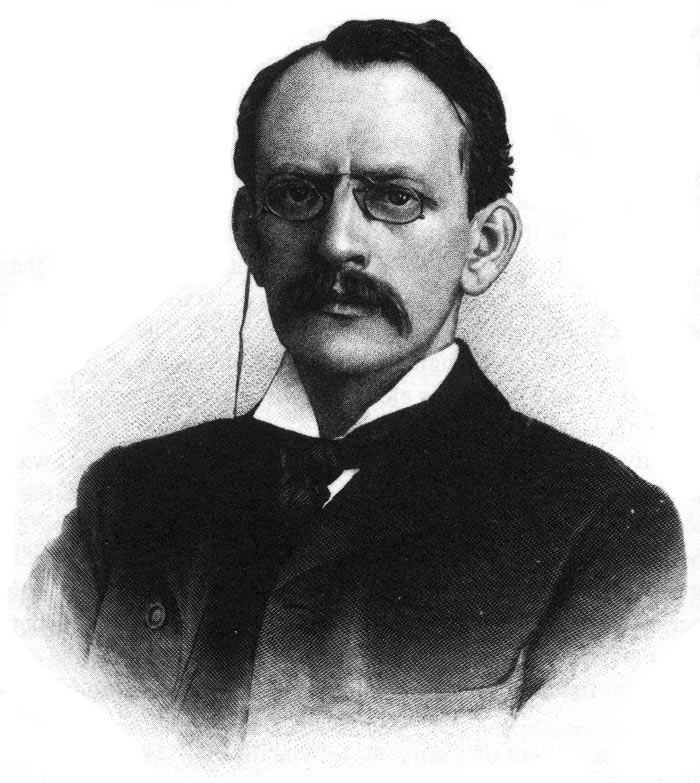
\includegraphics[width=0.92\textwidth]{images/thomson.jpg}
\captionof{figure}{J.~J.~Thomson (1856--1940).}
\end{minipage}\hfill
\begin{minipage}{0.30\textwidth}
\centering
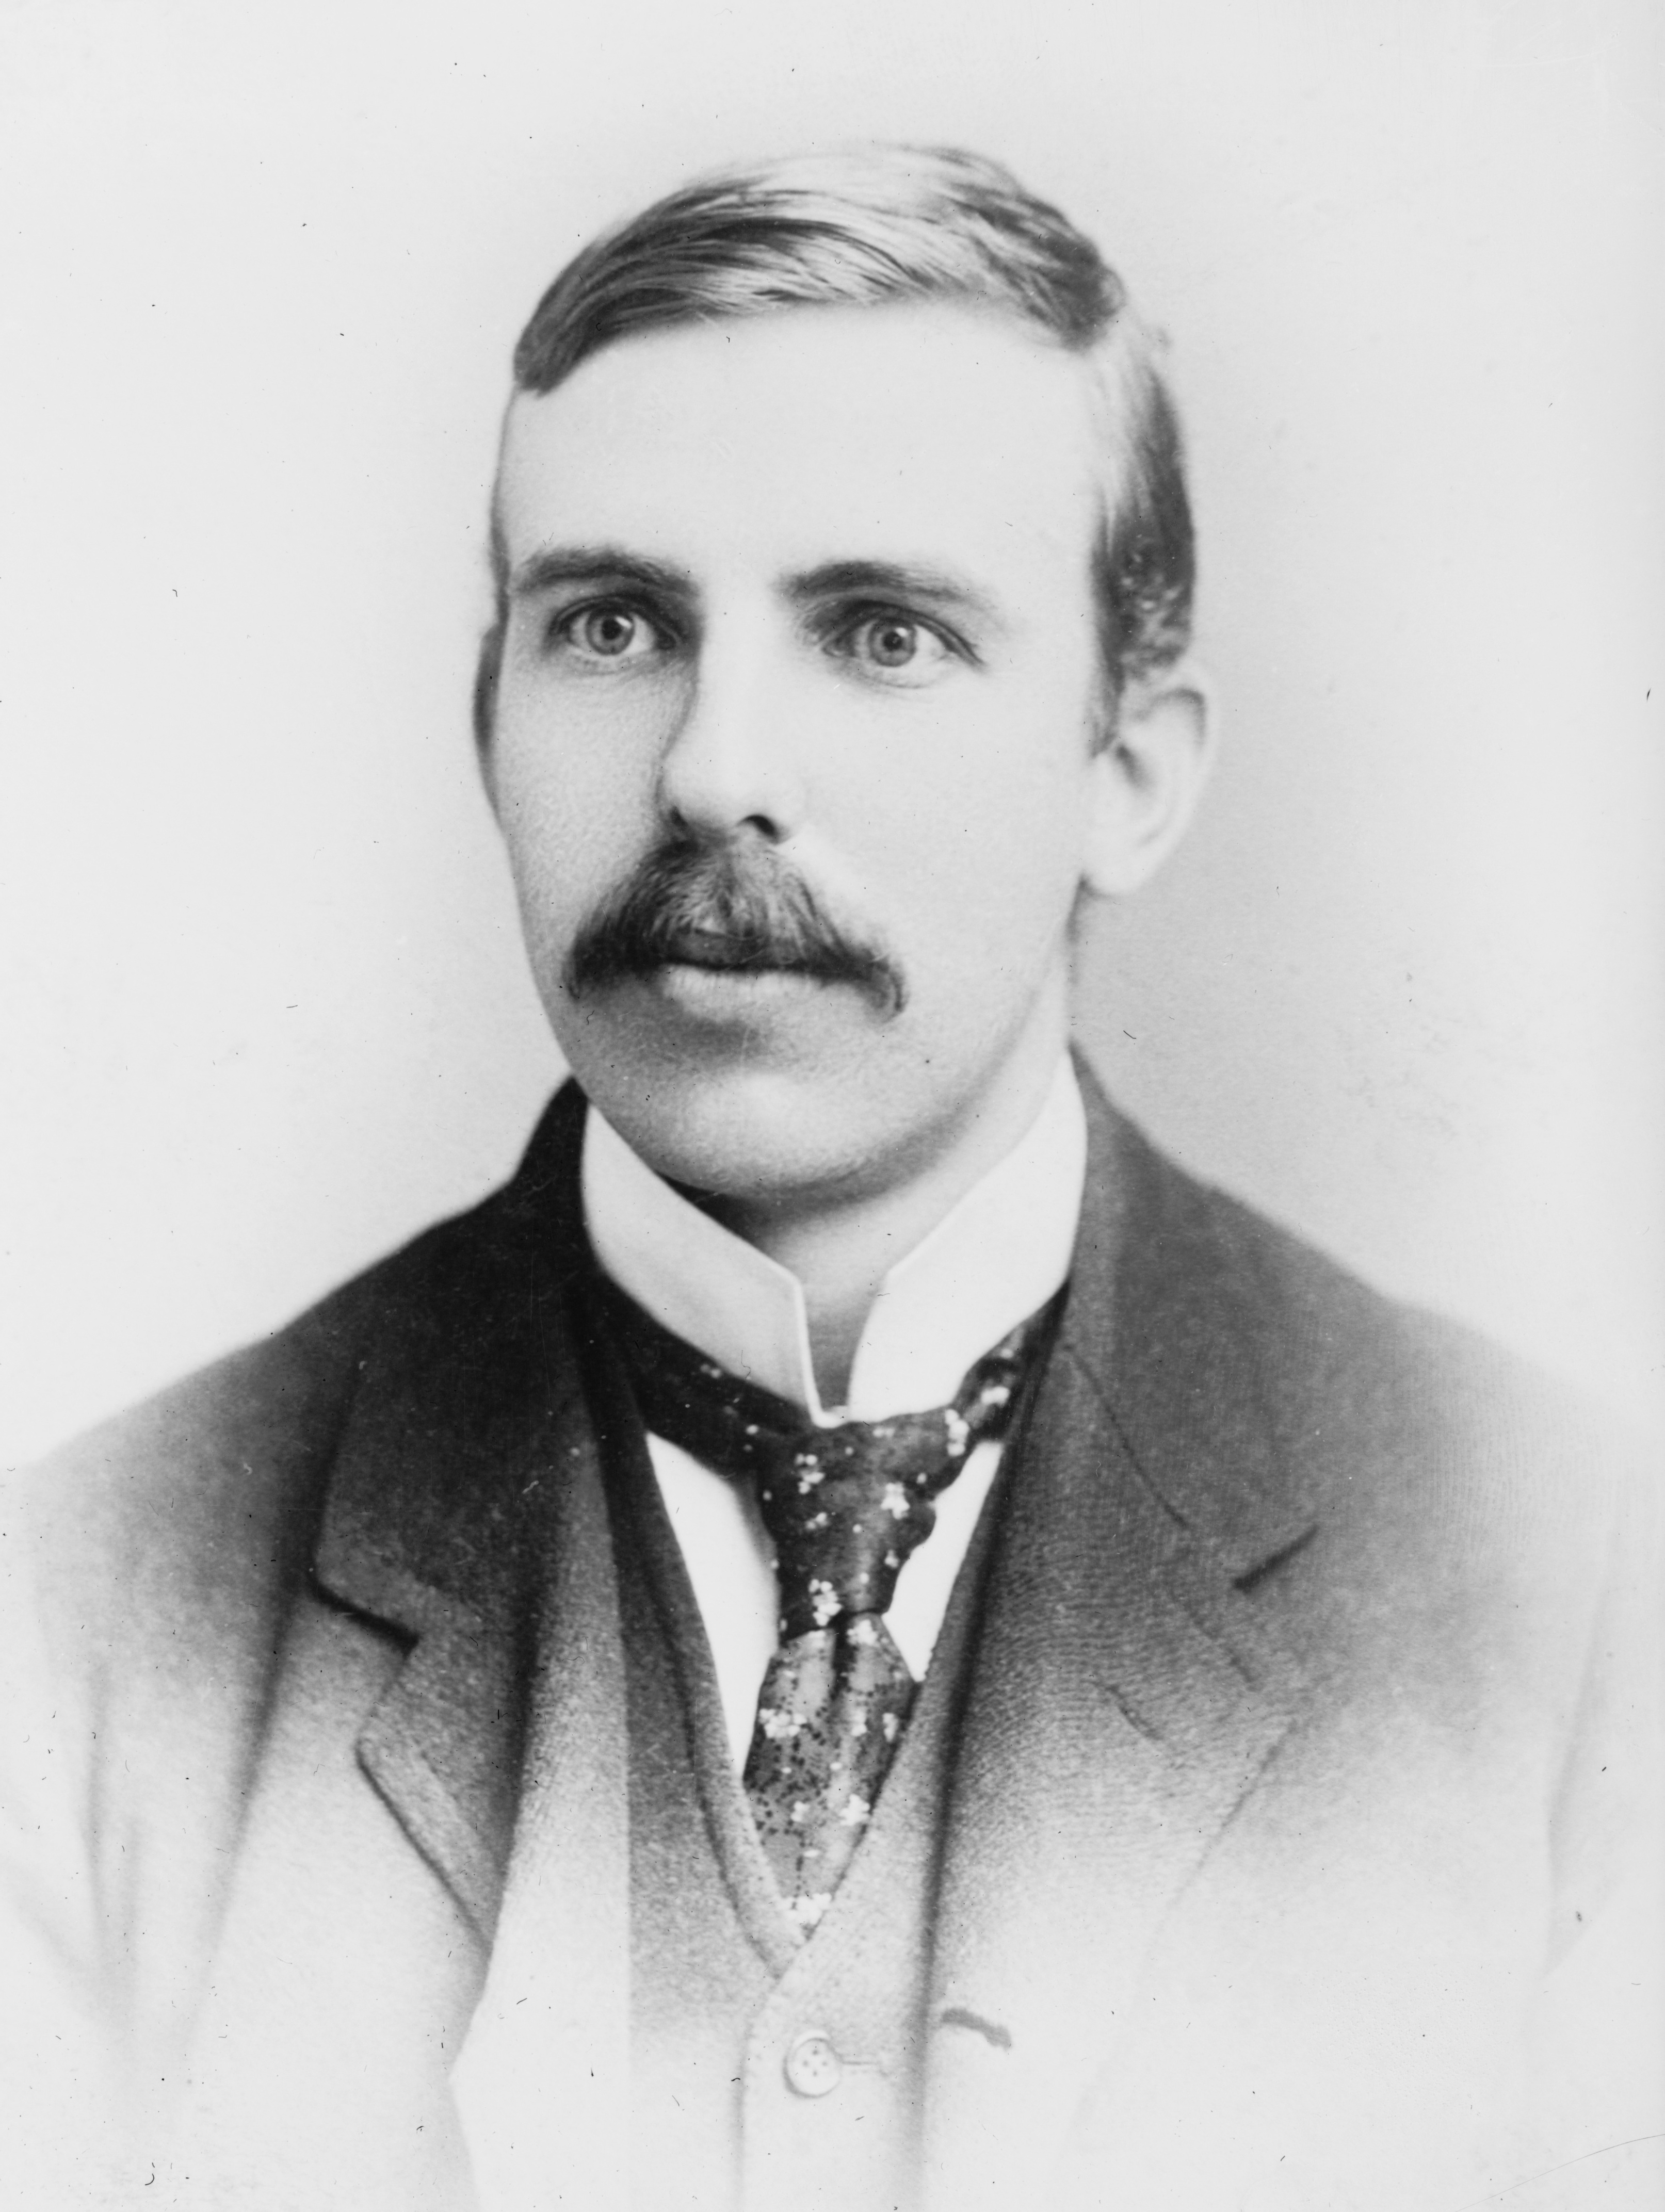
\includegraphics[width=0.92\textwidth]{images/rutherford.jpg}
\captionof{figure}{Ernest Rutherford (1871--1937).}
\end{minipage}\hfill
\begin{minipage}{0.30\textwidth}
\centering
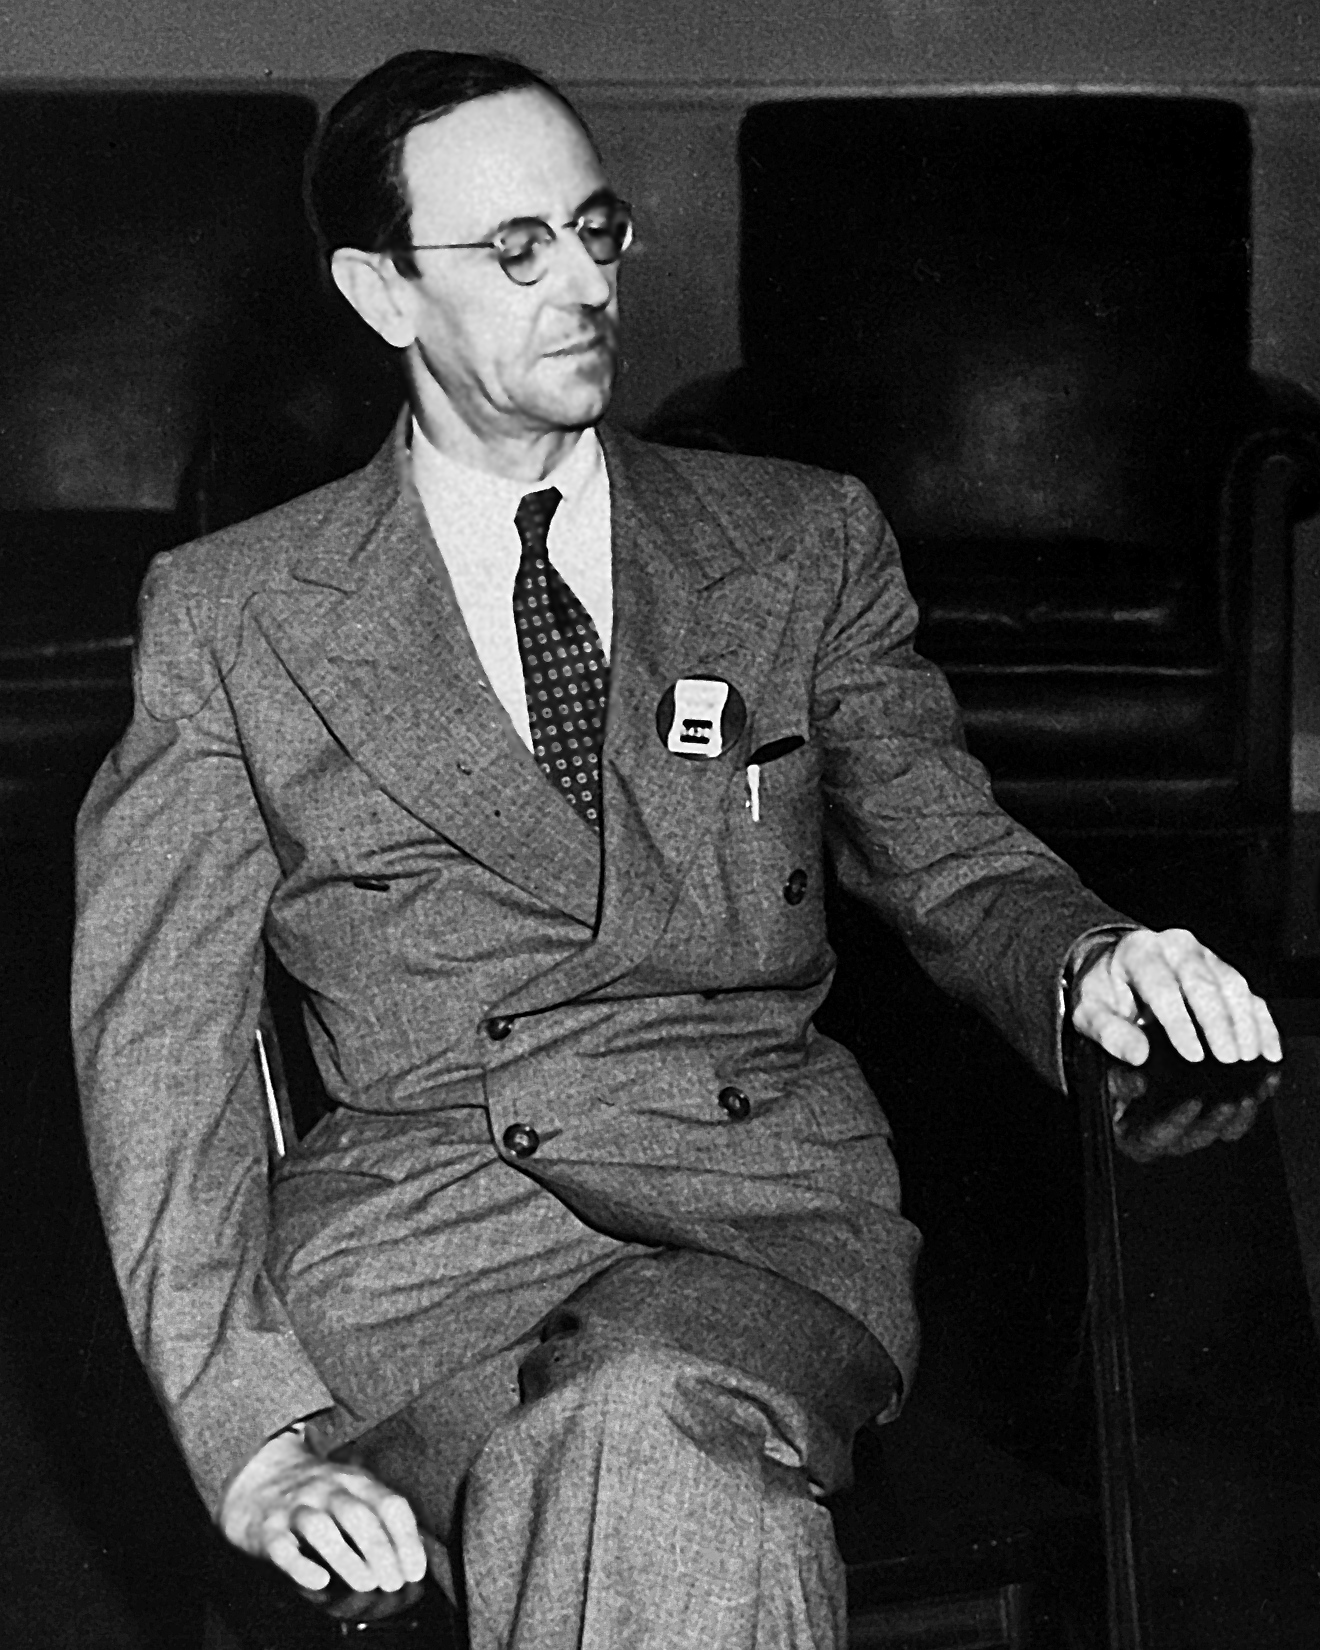
\includegraphics[width=0.92\textwidth]{images/chadwick.jpg}
\captionof{figure}{James Chadwick (1891--1974).}
\end{minipage}

Across four decades of extraordinary experimental physics at Cambridge University's Cavendish Laboratory, J.~J.~Thomson discovered the first fundamental particle (the electron, 1897); his student Ernest Rutherford discovered the atomic nucleus (1911) and the proton (1919); and Rutherford's student James Chadwick discovered the neutron (1932), establishing the modern physical model of the atom.
\end{historicalbox}

\begin{table}[htbp]
\centering
\renewcommand{\arraystretch}{1.35}
\begin{tabular}{@{}llllll@{}}
\toprule
\textbf{Particle} & \textbf{Symbol} & \textbf{Electric Charge (C)} & \textbf{Relative Charge} & \textbf{Rest Mass (kg)} & \textbf{Rest Mass (u)} \\
\midrule
\textbf{Proton} & $p$ (or $^1_1p$) & $+1.602\,176\,634 \times 10^{-19}$ & $+1$ & $1.672\,622 \times 10^{-27}$ & $1.007\,276\ \mathrm{u}$ \\
\textbf{Neutron} & $n$ (or $^1_0n$) & $0$ & $0$ & $1.674\,927 \times 10^{-27}$ & $1.008\,665\ \mathrm{u}$ \\
\textbf{Electron} & $e^-$ (or $^0_{-1}e$) & $-1.602\,176\,634 \times 10^{-19}$ & $-1$ & $9.109\,384 \times 10^{-31}$ & $0.000\,549\ \mathrm{u}$ \\
\bottomrule
\end{tabular}
\caption{Fundamental physical constants of the three subatomic constituents of matter.}
\label{tab:subatomic_particles}
\end{table}

\section{Nuclide Representation and Electronic Accounting}

\begin{definitionbox}{Standard Symbolic Representation of a Nuclide}
A specific nuclear species (a \textbf{nuclide}) of chemical element $\mathrm{X}$ is designated by the standardized IUPAC notation:
\begin{equation}
\ce{^{A}_{Z}X^{\pm q}},
\end{equation}
where:
\begin{itemize}[leftmargin=1.5em,itemsep=3pt]
  \item $Z$ is the \textbf{atomic number} (or \emph{charge number}), denoting the exact number of protons in the nucleus. It uniquely establishes the chemical identity and placement of the element in the periodic table.
  \item $A$ is the \textbf{mass number}, denoting the total integer count of nucleons (protons plus neutrons) in the nucleus:
  \begin{equation}
  A = Z + N.
  \end{equation}
  \item $N = A - Z$ is the number of neutrons.
  \item $\pm q$ is the net ionic charge (in units of elementary charge $e$).
\end{itemize}
\end{definitionbox}

\begin{lawbox}{Electronic Accounting in Atoms and Ions}
For any nuclide species $\ce{^{A}_{Z}X^{\pm q}}$:
\begin{enumerate}[leftmargin=1.5em,itemsep=3pt]
  \item \textbf{Electrically Neutral Atom ($q = 0$):} The positive nuclear charge is balanced by an identical number of surrounding orbital electrons:
  \begin{equation}
  N_{e^-} = Z.
  \end{equation}
  \item \textbf{Cation ($\ce{X^{q+}}$ with $q > 0$):} Formed when an atom loses $q$ valence electrons. The electron count is reduced:
  \begin{equation}
  N_{e^-} = Z - q.
  \end{equation}
  \item \textbf{Anion ($\ce{X^{q-}}$ with $q > 0$):} Formed when an atom gains $q$ additional electrons. The electron count is increased:
  \begin{equation}
  N_{e^-} = Z + q.
  \end{equation}
\end{enumerate}
\end{lawbox}

\section{Isotopes, Mass Spectrometry, and Relative Atomic Mass}

\subsection{Definition of Isotopes}
\begin{definitionbox}{Isotopes}
\textbf{Isotopes} are nuclides of the same chemical element that possess the **same atomic number $Z$** (identical proton and electron counts, hence identical chemical reactivity), but **different mass numbers $A$** (different numbers of neutrons $N$).
\end{definitionbox}

Because isotopes share identical chemical properties, they cannot be separated by standard chemical reactions; separation requires physical mass-dependent techniques such as **mass spectrometry**, gaseous diffusion, or ultracentrifugation.

\begin{historicalbox}{Francis William Aston and the Mass Spectrograph}
\begin{minipage}{0.28\textwidth}
\centering
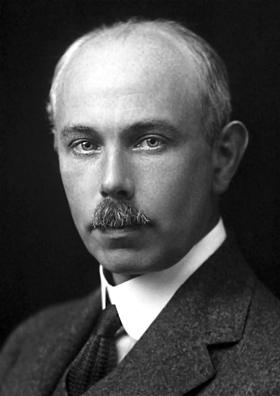
\includegraphics[width=0.92\textwidth]{images/aston.jpg}
\captionof{figure}{Francis William Aston (1877--1945), Nobel Prize in Chemistry 1922.}
\end{minipage}\hfill
\begin{minipage}{0.68\textwidth}
Working at the Cavendish Laboratory, British chemist and physicist Francis William Aston invented the electromagnetic **mass spectrograph** in 1919. By ionizing gas atoms and passing them through coordinated electric and magnetic fields, Aston focused ions of differing mass-to-charge ratios ($m/q$) onto distinct photographic lines.

Aston discovered 212 of the 287 naturally occurring stable isotopes, proving that non-integer elemental atomic weights (such as chlorine at $35.45\ \mathrm{u}$) arise naturally from weighted statistical mixtures of integer-mass isotopes ($^{35}\mathrm{Cl}$ and $^{37}\mathrm{Cl}$), formulating the **Whole Number Rule**.
\end{minipage}
\end{historicalbox}

\subsection{Canonical Isotopic Families}
\begin{itemize}[leftmargin=1.5em,itemsep=3pt]
  \item \textbf{Hydrogen Isotopes:}
  \begin{itemize}[leftmargin=1.2em]
    \item \textbf{Protium} ($\ce{^1_1H}$): $1\ p^+, 0\ n^0, 1\ e^-$ ($99.985\%$ natural terrestrial abundance).
    \item \textbf{Deuterium} ($\ce{^2_1H}$ or $\mathrm{D}$): $1\ p^+, 1\ n^0, 1\ e^-$ ($0.015\%$, stable; forms heavy water $\mathrm{D_2O}$).
    \item \textbf{Tritium} ($\ce{^3_1H}$ or $\mathrm{T}$): $1\ p^+, 2\ n^0, 1\ e^-$ (unstable, radioactive beta emitter, $t_{1/2} = 12.32\ \mathrm{yr}$).
  \end{itemize}
  \item \textbf{Carbon Isotopes:}
  \begin{itemize}[leftmargin=1.2em]
    \item $\ce{^{12}_6C}$: $6\ p^+, 6\ n^0$ ($98.93\%$ natural abundance; SI atomic mass definition standard).
    \item $\ce{^{13}_6C}$: $6\ p^+, 7\ n^0$ ($1.07\%$ natural abundance; nonzero nuclear spin $I = 1/2$, active in NMR spectroscopy).
    \item $\ce{^{14}_6C}$: $6\ p^+, 8\ n^0$ (radioactive trace $\sim 1.2 \times 10^{-12}$, used in radiocarbon archaeological dating).
  \end{itemize}
\end{itemize}

\subsection{Relative Average Atomic Mass}
In nature, an element $\mathrm{X}$ exists as a stable mixture of $k$ isotopes, each possessing a precise rest mass $m_i$ and a fractional natural abundance $x_i \in [0, 1]$ (or percentage abundance $\alpha_i = x_i \times 100\%$):

\begin{lawbox}{Average Relative Atomic Mass Formula}
The macroscopic average atomic mass $m_a$ (and molar mass $M$) of an element is the abundance-weighted arithmetic mean over all its natural isotopes:
\begin{equation}
m_a = \sum_{i=1}^k x_i \cdot m_i = \frac{\sum_{i=1}^k \alpha_i \cdot m_i}{\sum_{i=1}^k \alpha_i} = \frac{\sum_{i=1}^k \alpha_i \cdot m_i}{100\%},
\end{equation}
where $\sum_{i=1}^k x_i \equiv 1$ and $\sum_{i=1}^k \alpha_i \equiv 100\%$.
\end{lawbox}

\section{Nuclear Cohesion, Mass Defect, and Binding Energy}

\subsection{1. The Phenomenon of Mass Defect}
When isolated, unbound nucleons (protons and neutrons) coalesce under the strong nuclear force to assemble a bound atomic nucleus, high-precision mass spectrometry reveals that **the mass of the bound nucleus $M_{\text{nucleus}}$ is strictly and measurably less than the sum of the masses of its constituent free nucleons**:
\begin{equation}
M_{\text{nucleus}} < Z \cdot m_p + (A - Z) \cdot m_n.
\end{equation}

\begin{definitionbox}{Nuclear Mass Defect ($\Delta m$)}
The \textbf{mass defect} $\Delta m$ of a nucleus $\ce{^{A}_{Z}X}$ is defined as the positive difference between the total mass of its separated free nucleons and the actual mass of the assembled bound nucleus:
\begin{equation}
\Delta m \eqdef \left[ Z \cdot m_p + (A - Z) \cdot m_n \right] - M_{\text{nucleus}} > 0.
\end{equation}
Because laboratory tables list neutral atomic masses $M_{\text{atom}}(\ce{^{A}_{Z}X})$ rather than bare nuclear masses, adding $Z$ electron masses to both terms yields the equivalent atomic formulation:
\begin{equation}
\Delta m = \left[ Z \cdot m(\ce{^1_1H}) + (A - Z) \cdot m_n \right] - M_{\text{atom}}(\ce{^{A}_{Z}X}),
\end{equation}
where $m(\ce{^1_1H}) = m_p + m_e = 1.007\,825\ \mathrm{u}$ is the mass of a neutral hydrogen atom.
\end{definitionbox}

\begin{historicalbox}{Albert Einstein and the Mass-Energy Equivalence ($E = mc^2$)}
\begin{minipage}{0.28\textwidth}
\centering
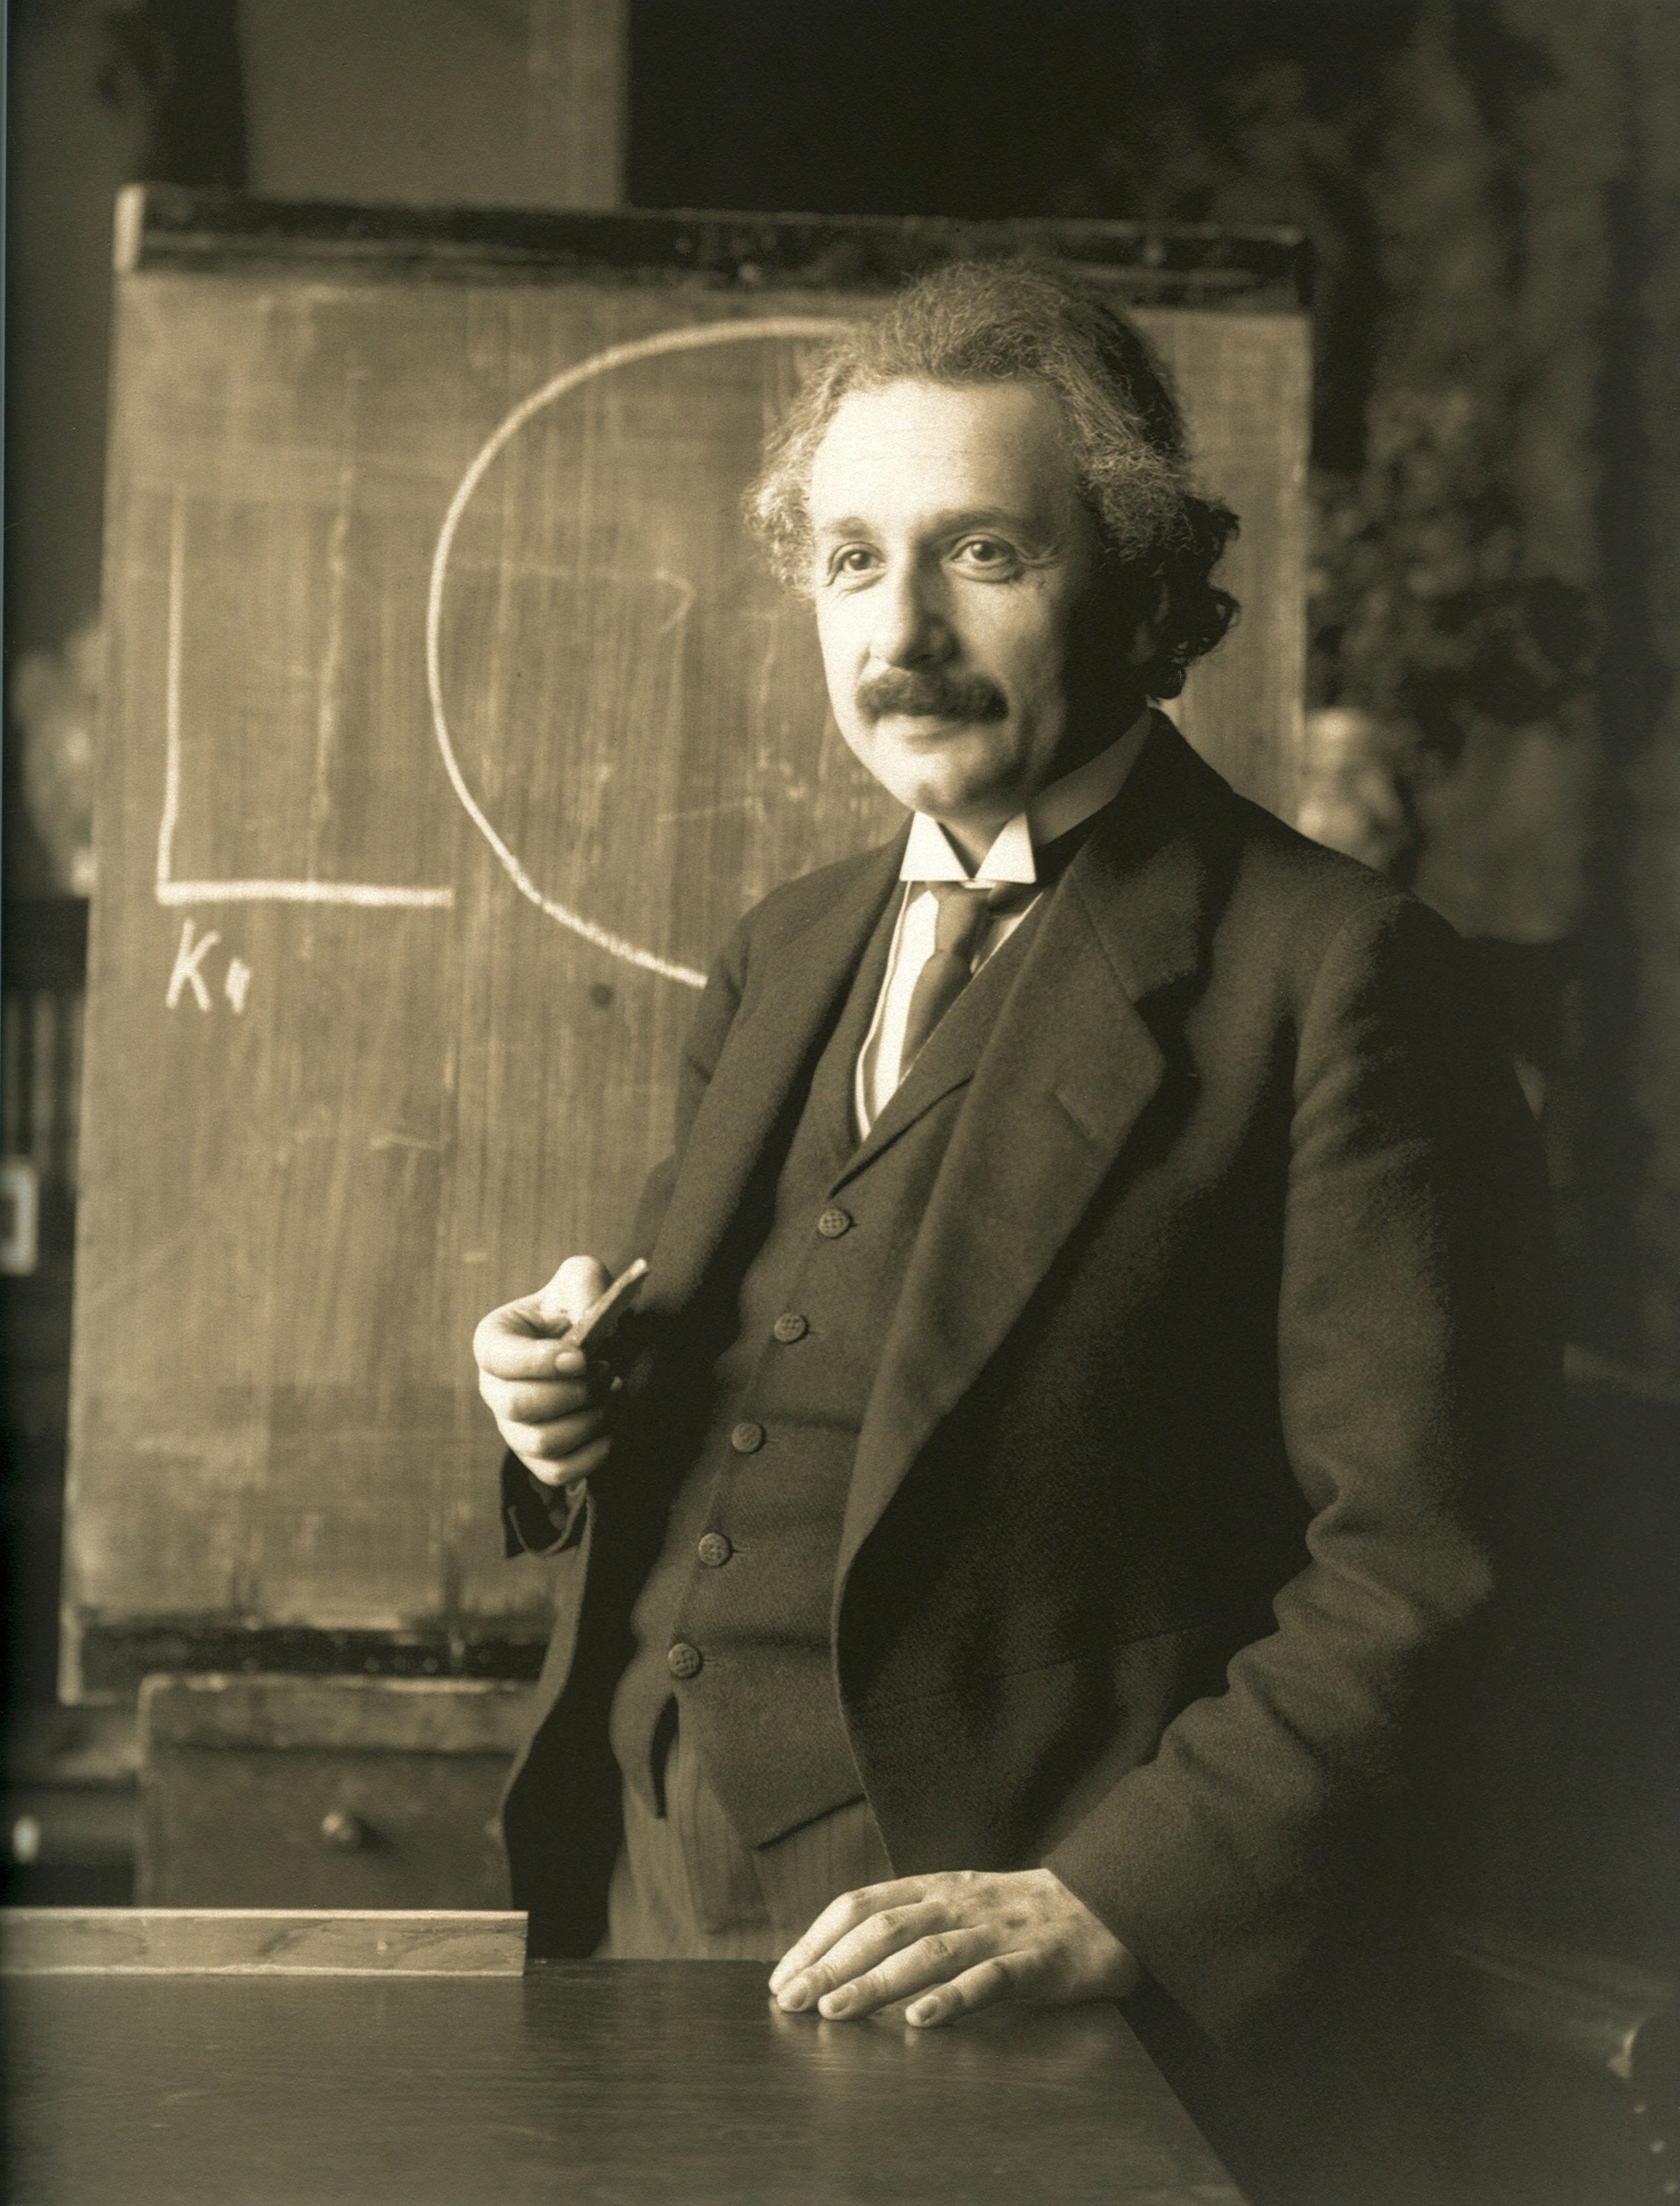
\includegraphics[width=0.92\textwidth]{images/einstein.jpg}
\captionof{figure}{Albert Einstein (1879--1955), portrait by Ferdinand Schmutzer (1921).}
\end{minipage}\hfill
\begin{minipage}{0.68\textwidth}
In September 1905, Albert Einstein published his fourth \emph{Annus Mirabilis} paper in \emph{Annalen der Physik}: ``\emph{Does the Inertia of a Body Depend upon its Energy Content?}'' 

Einstein deduced that mass is not an immutable substance, but concentrated potential energy:
\[
E = m \cdot c^2.
\]
The ``missing mass'' $\Delta m$ in atomic nuclei is converted during nuclear synthesis into binding energy, explaining why nuclear reactions release over \textbf{one million times} more energy per gram than any chemical combustion!
\end{minipage}
\end{historicalbox}

\subsection{2. Nuclear Binding Energy}

\begin{definitionbox}{Nuclear Binding Energy ($E_L$)}
The \textbf{binding energy} $E_L$ of a nucleus is defined as the minimum energy that must be supplied from the outside to dissociate the bound nucleus into its separate, non-interacting constituent nucleons at rest at infinity:
\begin{equation}
E_L \eqdef \Delta m \cdot c^2 > 0.
\end{equation}
Conversely, when free nucleons assemble to form the nucleus, an equivalent quantity of energy $\Delta E = -E_L < 0$ is released into the surroundings.
\end{definitionbox}

\subsection{3. Energy Conversion Factors}
In nuclear physics, energies are expressed in electronvolts ($\mathrm{eV}$) and mega-electronvolts ($\mathrm{MeV}$):
\begin{equation}
1\ \mathrm{eV} \eqdef 1.602\,176\,634 \times 10^{-19}\ \mathrm{J}, \qquad 1\ \mathrm{MeV} = 10^6\ \mathrm{eV} = 1.602\,176\,634 \times 10^{-13}\ \mathrm{J}.
\end{equation}
Using the speed of light in vacuum $c = 2.997\,924\,58 \times 10^8\ \mathrm{m\cdot s^{-1}}$, the energy equivalence of one atomic mass unit ($1\ \mathrm{u}$) is:
\[
E = (1.660\,539 \times 10^{-27}\ \mathrm{kg}) \times (2.997\,924\,58 \times 10^8\ \mathrm{m\cdot s^{-1}})^2 = 1.492\,418 \times 10^{-10}\ \mathrm{J}.
\]
Dividing by $1.602\,176\,634 \times 10^{-13}\ \mathrm{J/MeV}$:

\begin{lawbox}{The Universal Nuclear Conversion Constant}
\begin{equation}
1\ \mathrm{u} \cdot c^2 = \mathbf{931.494\ \mathrm{MeV}} \quad (\text{often rounded to } 931.5\ \mathrm{MeV}).
\end{equation}
Therefore, given mass defect $\Delta m$ directly in atomic mass units ($\mathrm{u}$):
\begin{equation}
E_L\ [\mathrm{MeV}] = \Delta m\ [\mathrm{u}] \times 931.494\ \mathrm{MeV\cdot u^{-1}}.
\end{equation}
\end{lawbox}

\section{Nuclear Stability and the Aston Curve}

While total binding energy $E_L$ increases monotonically with the total number of nucleons $A$, it does not measure the \emph{intrinsic stability} of a nucleus: a large nucleus like Uranium-238 has $E_L \approx 1800\ \mathrm{MeV}$, yet it is unstable and radioactively decays, while Iron-56 has $E_L \approx 492\ \mathrm{MeV}$ and is completely stable.

\begin{definitionbox}{Binding Energy per Nucleon ($E_L / A$)}
The true physical measure of nuclear cohesion and stability is the **binding energy per nucleon** (or \emph{specific binding energy}):
\begin{equation}
\frac{E_L}{A} \eqdef \frac{\Delta m \cdot c^2}{A}, \qquad \left[\frac{E_L}{A}\right] = \mathrm{MeV\cdot nucleon^{-1}}.
\end{equation}
The higher the value of $E_L / A$, the more tightly bound each nucleon is, and the more stable the atomic nucleus.
\end{definitionbox}

\begin{figure}[htbp]
\centering
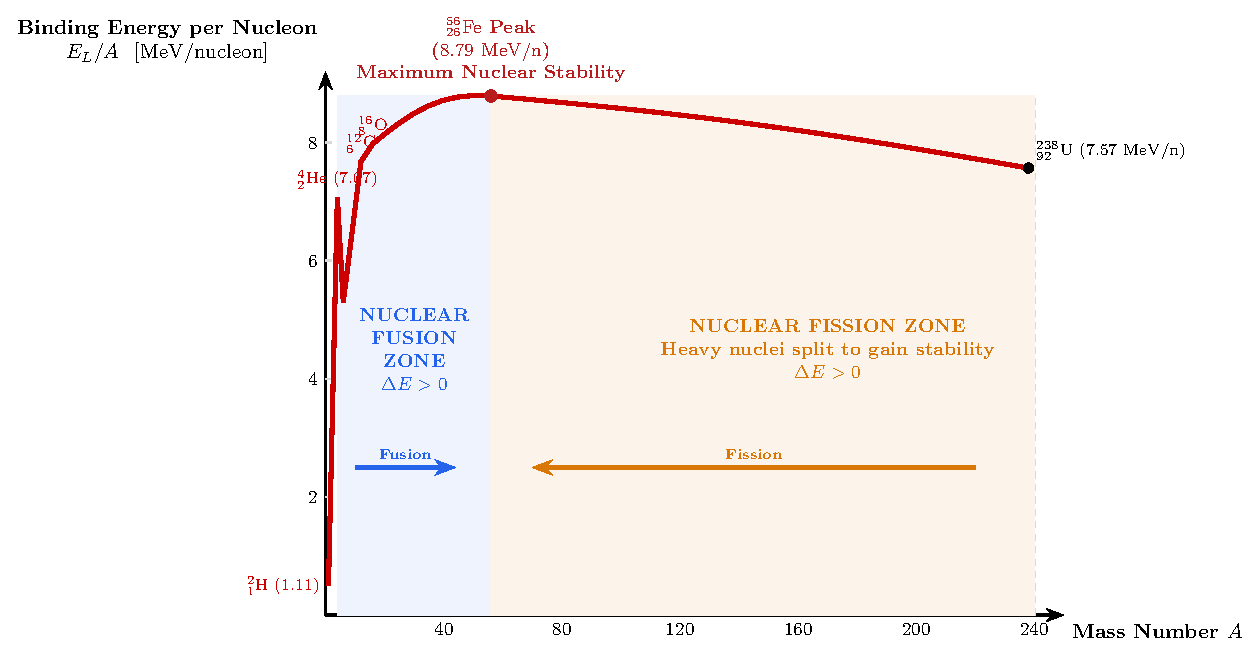
\includegraphics[width=0.88\textwidth]{figures/05_aston_curve.pdf}
\caption{The Aston Binding Energy Curve ($E_L / A$ versus mass number $A$). Nuclear stability peaks at Iron-56 ($^{56}_{26}\mathrm{Fe}$, $8.79\ \mathrm{MeV/nucleon}$). Exothermic nuclear fusion occurs for light nuclei ($A < 56$), while exothermic nuclear fission occurs for heavy nuclei ($A > 56$).}
\label{fig:aston_curve}
\end{figure}

\subsection{Thermodynamic Analysis of the Aston Curve}
The Aston curve exhibits three profound structural zones:
\begin{enumerate}[leftmargin=1.5em,itemsep=4pt]
  \item \textbf{Rapid Rise for Light Nuclei ($A < 20$):}
  The binding energy per nucleon rises steeply from $1.11\ \mathrm{MeV/n}$ in deuterium ($\ce{^2_1H}$) up to $\approx 8\ \mathrm{MeV/n}$. Pronounced local maxima occur at $\alpha$-conjugate nuclei ($\ce{^4_2He}$ at $7.07\ \mathrm{MeV/n}$, $\ce{^{12}_6C}$ at $7.68\ \mathrm{MeV/n}$, $\ce{^{16}_8O}$ at $7.98\ \mathrm{MeV/n}$), corresponding to filled nuclear energy shells.
  \item \textbf{The Iron Peak of Maximum Stability ($A \approx 56\text{--}62$):}
  The curve attains its global maximum at:
  \begin{equation}
  \left(\frac{E_L}{A}\right)_{\max} \approx 8.79\ \mathrm{MeV\cdot nucleon^{-1}} \quad \text{for } \ce{^{56}_{26}Fe} \text{ and } \ce{^{62}_{28}Ni}.
  \end{equation}
  Iron-56 and Nickel-62 are the most thermodynamically stable nuclei in the universe. They represent the final energetic endpoint of stellar nucleosynthesis in massive stars.
  \item \textbf{Gradual Decline for Heavy Nuclei ($A > 60$):}
  Beyond iron, $E_L / A$ gradually drops to $7.57\ \mathrm{MeV/n}$ for Uranium-238 ($\ce{^{238}_{92}U}$). This decrease is driven by the long-range electrostatic Coulomb repulsion between protons ($V_C \propto Z^2/R$), which scales faster than the short-range strong nuclear attraction.
\end{enumerate}

\begin{lawbox}{Thermodynamics of Nuclear Energy: Fusion vs. Fission}
Any nuclear transformation that moves a system toward the Iron Peak ($\ce{^{56}Fe}$) increases binding energy per nucleon and is **strongly exothermic** ($\Delta E_{\text{reaction}} > 0$):
\begin{itemize}[leftmargin=1.5em,itemsep=3pt]
  \item \textbf{Thermonuclear Fusion ($A \ll 56$):} Combining two light nuclei with low $E_L / A$ into a heavier nucleus with higher $E_L / A$ releases enormous energy:
  \[
  \ce{^2_1H + ^3_1H -> ^4_2He + ^1_0n} + 17.59\ \mathrm{MeV}.
  \]
  \item \textbf{Nuclear Fission ($A \gg 56$):} Splitting a massive nucleus with lower $E_L / A$ into two intermediate nuclei with higher $E_L / A$ releases energy:
  \[
  \ce{^{235}_{92}U + ^1_0n -> ^{141}_{56}Ba + ^{92}_{36}Kr + 3\,^1_0n} + 200\ \mathrm{MeV}.
  \]
\end{itemize}
\end{lawbox}

\section{Comprehensive Worked Examples}

\begin{workedexample}{Subatomic Accounting of Neutral Atoms and Complex Ions}
Determine the number of protons ($p^+$), neutrons ($n^0$), and electrons ($e^-$), as well as the total nuclear charge $Q_{\text{nucleus}}$ and electronic cloud charge $Q_{\text{electrons}}$ for each of the following chemical species:
\begin{enumerate}[leftmargin=1.4em,itemsep=2pt]
  \item Neutral Iron-56 atom: $\ce{^{56}_{26}Fe}$,
  \item Ferric iron cation: $\ce{^{56}_{26}Fe^{3+}}$,
  \item Chloride anion: $\ce{^{35}_{17}Cl^-}$,
  \item Ammonium polyatomic cation: $\ce{^{14}_7N^1_1H_4^+}$,
  \item Phosphate polyatomic anion: $\ce{^{31}_{15}P^{16}_8O_4^{3-}}$.
\end{enumerate}

\paragraph{Solution.}
Using the rules: $Z = N_{p^+}$, $N = A - Z$, $N_{e^-} = Z - q$ (for charge $+q$) and $N_{e^-} = Z + q$ (for charge $-q$).
Elementary charge is $e = 1.602 \times 10^{-19}\ \mathrm{C}$.

\textbf{1. Neutral Iron-56 ($\ce{^{56}_{26}Fe}$):}\\
$Z = 26$, $A = 56$, $q = 0$.
\begin{itemize}[leftmargin=1.5em,itemsep=1pt]
  \item Protons: $N_{p^+} = Z = \mathbf{26}$.
  \item Neutrons: $N_{n^0} = A - Z = 56 - 26 = \mathbf{30}$.
  \item Electrons: $N_{e^-} = Z = \mathbf{26}$.
  \item $Q_{\text{nucleus}} = +26\,e = +4.165 \times 10^{-18}\ \mathrm{C}$; $Q_{\text{electrons}} = -26\,e = -4.165 \times 10^{-18}\ \mathrm{C}$ ($Q_{\text{net}} = 0$).
\end{itemize}

\textbf{2. Ferric Cation ($\ce{^{56}_{26}Fe^{3+}}$):}\\
$Z = 26$, $A = 56$, $q = +3$.
\begin{itemize}[leftmargin=1.5em,itemsep=1pt]
  \item Protons: $N_{p^+} = Z = \mathbf{26}$.
  \item Neutrons: $N_{n^0} = 56 - 26 = \mathbf{30}$.
  \item Electrons: $N_{e^-} = Z - 3 = 26 - 3 = \mathbf{23}$.
  \item Net charge: $Q_{\text{net}} = +3\,e = +4.806 \times 10^{-19}\ \mathrm{C}$.
\end{itemize}

\textbf{3. Chloride Anion ($\ce{^{35}_{17}Cl^-}$):}\\
$Z = 17$, $A = 35$, $q = -1$.
\begin{itemize}[leftmargin=1.5em,itemsep=1pt]
  \item Protons: $N_{p^+} = Z = \mathbf{17}$.
  \item Neutrons: $N_{n^0} = 35 - 17 = \mathbf{18}$.
  \item Electrons: $N_{e^-} = Z + 1 = 17 + 1 = \mathbf{18}$ (argon noble-gas configuration).
  \item Net charge: $Q_{\text{net}} = -1\,e = -1.602 \times 10^{-19}\ \mathrm{C}$.
\end{itemize}

\textbf{4. Ammonium Polyatomic Cation ($\ce{NH_4^+}$):}\\
Consists of one Nitrogen ($\ce{^{14}_7N}$) and four Hydrogens ($\ce{^1_1H}$), net charge $q = +1$.
\begin{itemize}[leftmargin=1.5em,itemsep=1pt]
  \item Total protons: $N_{p^+} = Z(\mathrm{N}) + 4 \times Z(\mathrm{H}) = 7 + 4(1) = \mathbf{11}$.
  \item Total neutrons: $N_{n^0} = (14 - 7) + 4 \times (1 - 1) = 7 + 0 = \mathbf{7}$.
  \item Total electrons: $N_{e^-} = N_{p^+} - 1 = 11 - 1 = \mathbf{10}$ (neon configuration).
\end{itemize}

\textbf{5. Phosphate Polyatomic Anion ($\ce{PO_4^{3-}}$):}\\
Consists of one Phosphorus ($\ce{^{31}_{15}P}$) and four Oxygens ($\ce{^{16}_8O}$), net charge $q = -3$.
\begin{itemize}[leftmargin=1.5em,itemsep=1pt]
  \item Total protons: $N_{p^+} = Z(\mathrm{P}) + 4 \times Z(\mathrm{O}) = 15 + 4(8) = 15 + 32 = \mathbf{47}$.
  \item Total neutrons: $N_{n^0} = (31 - 15) + 4 \times (16 - 8) = 16 + 4(8) = 16 + 32 = \mathbf{48}$.
  \item Total electrons: $N_{e^-} = N_{p^+} + 3 = 47 + 3 = \mathbf{50}$.
\end{itemize}
\end{workedexample}

\begin{workedexample}{Determination of Isotopic Abundances from Mass Spectrometry}
Natural copper ($\mathrm{Cu}$) consists of two stable isotopes: $\ce{^{63}_{29}Cu}$ and $\ce{^{65}_{29}Cu}$. High-resolution mass spectrometry gives their isotopic rest masses:
\[
m(\ce{^{63}Cu}) = 62.9296\ \mathrm{u}, \qquad m(\ce{^{65}Cu}) = 64.9278\ \mathrm{u}.
\]
The standard relative atomic mass of naturally occurring copper is $M(\mathrm{Cu}) = 63.5460\ \mathrm{u}$.
\begin{enumerate}[leftmargin=1.4em,itemsep=3pt]
  \item Calculate the fractional abundances ($x_1, x_2$) and percentage abundances ($\alpha_1, \alpha_2$) of the two isotopes in nature.
  \item For a pure foil of copper weighing $m_{\text{sample}} = 10.00\ \mathrm{g}$, calculate the total number of copper atoms, and the individual number of $\ce{^{63}Cu}$ and $\ce{^{65}Cu}$ atoms present.
\end{enumerate}

\paragraph{Solution.}
\textbf{1. Isotopic Abundance System of Equations:}\\
Let $x_1$ be the fractional abundance of $\ce{^{63}Cu}$ and $x_2$ be the fractional abundance of $\ce{^{65}Cu}$.
They satisfy the system of linear equations:
\[
\begin{cases}
x_1 + x_2 = 1 \implies x_2 = 1 - x_1, \\
x_1 \cdot m_1 + x_2 \cdot m_2 = M(\mathrm{Cu}).
\end{cases}
\]
Substituting $x_2 = 1 - x_1$:
\[
x_1 \cdot m_1 + (1 - x_1) \cdot m_2 = M(\mathrm{Cu}) \implies x_1(m_1 - m_2) + m_2 = M(\mathrm{Cu}).
\]
Solving for $x_1$:
\[
x_1 = \frac{m_2 - M(\mathrm{Cu})}{m_2 - m_1} = \frac{64.9278 - 63.5460}{64.9278 - 62.9296} = \frac{1.3818}{1.9982} \approx \mathbf{0.69152} = \mathbf{69.15\%}.
\]
Then $x_2$ is:
\[
x_2 = 1 - x_1 = 1 - 0.69152 = \mathbf{0.30848} = \mathbf{30.85\%}.
\]
Natural copper is composed of $69.15\%$ Copper-63 and $30.85\%$ Copper-65.

\textbf{2. Number of Atoms in the Sample:}\\
The amount of copper in $10.00\ \mathrm{g}$ is:
\[
n = \frac{m_{\text{sample}}}{M} = \frac{10.00\ \mathrm{g}}{63.5460\ \mathrm{g\cdot mol^{-1}}} \approx 0.15737\ \mathrm{mol}.
\]
The total number of copper atoms is:
\[
N_{\text{total}} = n \cdot N_A = 0.15737\ \mathrm{mol} \times 6.02214 \times 10^{23}\ \mathrm{mol^{-1}} \approx \mathbf{9.477 \times 10^{22}\ \text{atoms}}.
\]
The number of $\ce{^{63}Cu}$ atoms is:
\[
N(\ce{^{63}Cu}) = x_1 \cdot N_{\text{total}} = 0.69152 \times 9.477 \times 10^{22} \approx \mathbf{6.554 \times 10^{22}\ \text{atoms}}.
\]
The number of $\ce{^{65}Cu}$ atoms is:
\[
N(\ce{^{65}Cu}) = x_2 \cdot N_{\text{total}} = 0.30848 \times 9.477 \times 10^{22} \approx \mathbf{2.923 \times 10^{22}\ \text{atoms}}.
\]
\end{workedexample}

\begin{workedexample}{Nuclear Mass Defect and Binding Energy of Helium-4 and Iron-56}
Given the following ultra-precise rest masses:
\begin{align*}
\text{Proton mass } m_p &= 1.007\,276\ \mathrm{u}, & \text{Neutron mass } m_n &= 1.008\,665\ \mathrm{u}, \\
\text{Hydrogen atom } m(\ce{^1_1H}) &= 1.007\,825\ \mathrm{u}, & \text{Helium-4 atom } M(\ce{^4_2He}) &= 4.002\,603\ \mathrm{u}, \\
\text{Iron-56 atom } M(\ce{^{56}_{26}Fe}) &= 55.934\,937\ \mathrm{u}.
\end{align*}
\begin{enumerate}[leftmargin=1.4em,itemsep=3pt]
  \item Calculate the mass defect $\Delta m$ of Helium-4 in $\mathrm{u}$ and in kilograms ($\mathrm{kg}$).
  \item Compute the total binding energy $E_L$ of Helium-4 in $\mathrm{MeV}$ and in joules ($\mathrm{J}$), and find its binding energy per nucleon $E_L / A$.
  \item Calculate the mass defect $\Delta m$, total binding energy $E_L$, and specific binding energy $E_L / A$ of Iron-56 ($\ce{^{56}_{26}Fe}$).
  \item Compare the stability of Helium-4 and Iron-56.
\end{enumerate}

\paragraph{Solution.}
\textbf{1. Mass Defect of Helium-4 ($\ce{^4_2He}$):}\\
A neutral $\ce{^4_2He}$ atom consists of $Z = 2$ protons, $N = A - Z = 4 - 2 = 2$ neutrons, and $2$ electrons.
Using the neutral hydrogen atom formula:
\[
\Delta m(\ce{^4He}) = \left[ 2 \cdot m(\ce{^1H}) + 2 \cdot m_n \right] - M(\ce{^4He}).
\]
\[
\Delta m = \left[ 2(1.007\,825) + 2(1.008\,665) \right] - 4.002\,603 = [2.015\,650 + 2.017\,330] - 4.002\,603.
\]
\[
\Delta m = 4.032\,980 - 4.002\,603 = \mathbf{0.030\,377\ \mathrm{u}}.
\]
In kilograms:
\[
\Delta m = 0.030\,377\ \mathrm{u} \times 1.660\,539 \times 10^{-27}\ \mathrm{kg\cdot u^{-1}} \approx \mathbf{5.0442 \times 10^{-29}\ \mathrm{kg}}.
\]

\textbf{2. Binding Energy of Helium-4:}\\
Using the conversion factor $1\ \mathrm{u} \equiv 931.494\ \mathrm{MeV}$:
\[
E_L(\ce{^4He}) = 0.030\,377\ \mathrm{u} \times 931.494\ \mathrm{MeV\cdot u^{-1}} \approx \mathbf{28.296\ \mathrm{MeV}}.
\]
In joules:
\[
E_L = 28.296 \times 10^6\ \mathrm{eV} \times 1.602\,177 \times 10^{-19}\ \mathrm{J\cdot eV^{-1}} \approx \mathbf{4.533 \times 10^{-12}\ \mathrm{J}}.
\]
The binding energy per nucleon is ($A = 4$):
\[
\frac{E_L}{A} = \frac{28.296\ \mathrm{MeV}}{4} \approx \mathbf{7.074\ \mathrm{MeV\cdot nucleon^{-1}}}.
\]

\textbf{3. Binding Energy of Iron-56 ($\ce{^{56}_{26}Fe}$):}\\
For Iron-56 ($Z = 26$, $N = 56 - 26 = 30$):
\[
\Delta m(\ce{^{56}Fe}) = \left[ 26 \cdot m(\ce{^1H}) + 30 \cdot m_n \right] - M(\ce{^{56}Fe}).
\]
\[
26 \times 1.007\,825 = 26.203\,450\ \mathrm{u}, \qquad 30 \times 1.008\,665 = 30.259\,950\ \mathrm{u}.
\]
Total mass of separated nucleons:
\[
\sum m_{\text{nucleons}} = 26.203\,450 + 30.259\,950 = 56.463\,400\ \mathrm{u}.
\]
The mass defect is:
\[
\Delta m(\ce{^{56}Fe}) = 56.463\,400 - 55.934\,937 = \mathbf{0.528\,463\ \mathrm{u}}.
\]
In kilograms: $\Delta m = 0.528\,463 \times 1.6605 \times 10^{-27} \approx 8.775 \times 10^{-28}\ \mathrm{kg}$.
The total binding energy is:
\[
E_L(\ce{^{56}Fe}) = 0.528\,463\ \mathrm{u} \times 931.494\ \mathrm{MeV\cdot u^{-1}} \approx \mathbf{492.265\ \mathrm{MeV}}.
\]
The binding energy per nucleon is ($A = 56$):
\[
\frac{E_L}{A} = \frac{492.265\ \mathrm{MeV}}{56} \approx \mathbf{8.790\ \mathrm{MeV\cdot nucleon^{-1}}}.
\]

\textbf{4. Stability Comparison:}\\
Because $\frac{E_L}{A}(\ce{^{56}Fe}) = 8.79\ \mathrm{MeV/n} > \frac{E_L}{A}(\ce{^4He}) = 7.07\ \mathrm{MeV/n}$, the nucleons in Iron-56 are substantially more tightly bound than those in Helium-4. Iron-56 represents the pinnacle of nuclear stability.
\end{workedexample}

\begin{workedexample}{Energetics of Induced Nuclear Fission vs. Thermonuclear Fusion}
Compare the energy yields of nuclear fission and fusion:
\begin{enumerate}[leftmargin=1.4em,itemsep=3pt]
  \item Consider the thermal neutron-induced fission of Uranium-235:
  \[
  \ce{^{235}_{92}U + ^1_0n -> ^{141}_{56}Ba + ^{92}_{36}Kr + 3\,^1_0n}.
  \]
  Given the isotopic masses:
  $m(\ce{^{235}U}) = 235.043\,929\ \mathrm{u}$, $m(\ce{^{141}Ba}) = 140.914\,411\ \mathrm{u}$, $m(\ce{^{92}Kr}) = 91.926\,156\ \mathrm{u}$, and $m_n = 1.008\,665\ \mathrm{u}$.
  Calculate the mass variation $\Delta M$, the energy released $\Delta E$ per fission event (in $\mathrm{MeV}$ and $\mathrm{J}$), and the specific energy yield per kilogram of Uranium-235 ($\mathrm{J\cdot kg^{-1}}$).
  \item Consider the Deuterium-Tritium ($\mathrm{D}$-$\mathrm{T}$) thermonuclear fusion:
  \[
  \ce{^2_1H + ^3_1H -> ^4_2He + ^1_0n}.
  \]
  Given: $m(\ce{^2H}) = 2.014\,102\ \mathrm{u}$, $m(\ce{^3H}) = 3.016\,049\ \mathrm{u}$, $m(\ce{^4He}) = 4.002\,603\ \mathrm{u}$.
  Calculate the energy released $\Delta E$ per fusion event (in $\mathrm{MeV}$), and the specific energy yield per kilogram of $\mathrm{D}$-$\mathrm{T}$ fuel mix ($\mathrm{J\cdot kg^{-1}}$).
  \item Compare both nuclear yields to the chemical combustion of high-grade coal ($3.0 \times 10^7\ \mathrm{J\cdot kg^{-1}}$).
\end{enumerate}

\paragraph{Solution.}
\textbf{1. Fission Energetics:}\\
Initial reactant mass:
\[
M_{\text{initial}} = m(\ce{^{235}U}) + m_n = 235.043\,929 + 1.008\,665 = 236.052\,594\ \mathrm{u}.
\]
Final product mass:
\[
M_{\text{final}} = m(\ce{^{141}Ba}) + m(\ce{^{92}Kr}) + 3\,m_n = 140.914\,411 + 91.926\,156 + 3(1.008\,665) = 235.866\,562\ \mathrm{u}.
\]
Mass defect of the reaction:
\[
\Delta M_{\text{fission}} = M_{\text{initial}} - M_{\text{final}} = 236.052\,594 - 235.866\,562 = \mathbf{0.186\,032\ \mathrm{u}}.
\]
The energy released per single fission event is:
\[
\Delta E_{\text{fission}} = 0.186\,032\ \mathrm{u} \times 931.494\ \mathrm{MeV\cdot u^{-1}} \approx \mathbf{173.29\ \mathrm{MeV}}.
\]
In joules:
\[
\Delta E_{\text{fission}} = 173.29 \times 10^6 \times 1.6022 \times 10^{-19}\ \mathrm{J} \approx \mathbf{2.776 \times 10^{-11}\ \mathrm{J}}.
\]
One kilogram of pure $\ce{^{235}U}$ contains:
\[
N = \frac{1000\ \mathrm{g}}{235.04\ \mathrm{g\cdot mol^{-1}}} \times 6.022 \times 10^{23}\ \mathrm{mol^{-1}} \approx 2.562 \times 10^{24}\ \text{nuclei}.
\]
The specific energy yield of Uranium-235 fission is:
\[
\mathcal{E}_{\text{fission}} = (2.562 \times 10^{24}) \times (2.776 \times 10^{-11}\ \mathrm{J}) \approx \mathbf{7.11 \times 10^{13}\ \mathrm{J\cdot kg^{-1}} = 71.1\ \mathrm{TJ\cdot kg^{-1}}}.
\]

\textbf{2. D-T Fusion Energetics:}\\
Initial reactant mass:
\[
M_{\text{initial}} = m(\ce{^2H}) + m(\ce{^3H}) = 2.014\,102 + 3.016\,049 = 5.030\,151\ \mathrm{u}.
\]
Final product mass:
\[
M_{\text{final}} = m(\ce{^4He}) + m_n = 4.002\,603 + 1.008\,665 = 5.011\,268\ \mathrm{u}.
\]
Mass defect of fusion:
\[
\Delta M_{\text{fusion}} = 5.030\,151 - 5.011\,268 = \mathbf{0.018\,883\ \mathrm{u}}.
\]
Energy released per single fusion event:
\[
\Delta E_{\text{fusion}} = 0.018\,883\ \mathrm{u} \times 931.494\ \mathrm{MeV\cdot u^{-1}} \approx \mathbf{17.59\ \mathrm{MeV}}.
\]
In joules:
\[
\Delta E_{\text{fusion}} = 17.59 \times 10^6 \times 1.6022 \times 10^{-19}\ \mathrm{J} \approx \mathbf{2.818 \times 10^{-12}\ \mathrm{J}}.
\]
The molar mass of the stoichiometric $\mathrm{D}$-$\mathrm{T}$ reaction pair is:
\[
M_{\text{pair}} \approx 2.014 + 3.016 = 5.030\ \mathrm{g\cdot mol^{-1}}.
\]
One kilogram of $\mathrm{D}$-$\mathrm{T}$ fuel contains:
\[
N_{\text{pairs}} = \frac{1000\ \mathrm{g}}{5.030\ \mathrm{g\cdot mol^{-1}}} \times 6.022 \times 10^{23}\ \mathrm{mol^{-1}} \approx 1.197 \times 10^{26}\ \text{pairs}.
\]
The specific energy yield of $\mathrm{D}$-$\mathrm{T}$ fusion is:
\[
\mathcal{E}_{\text{fusion}} = (1.197 \times 10^{26}) \times (2.818 \times 10^{-12}\ \mathrm{J}) \approx \mathbf{3.37 \times 10^{14}\ \mathrm{J\cdot kg^{-1}} = 337\ \mathrm{TJ\cdot kg^{-1}}}.
\]

\textbf{3. Comparison with Chemical Combustion:}\\
\begin{itemize}[leftmargin=1.5em,itemsep=2pt]
  \item Coal combustion: $\mathcal{E}_{\text{coal}} \approx 3.0 \times 10^7\ \mathrm{J\cdot kg^{-1}} = 30\ \mathrm{MJ\cdot kg^{-1}}$.
  \item Fission of $\ce{^{235}U}$: $7.11 \times 10^{13}\ \mathrm{J\cdot kg^{-1}} \implies \mathbf{2.37 \times 10^6}$ times more energy than coal!
  \item Fusion of $\mathrm{D}$-$\mathrm{T}$: $3.37 \times 10^{14}\ \mathrm{J\cdot kg^{-1}} \implies \mathbf{11.2 \times 10^6}$ times more energy than coal, and nearly $5\times$ more energy per kilogram than uranium fission!
\end{itemize}
\end{workedexample}
